% !TEX TS-program = xelatex
% !TEX encoding = UTF-8
\documentclass[onecolumn,oneside]{SUSTechHomework}
\usepackage{graphicx}

\author{董骏博}
\sid{12432995}
\title{Homework 1}
\coursecode{CSE5001}
\coursename{Advanced Artificial Intelligence Fall 2024}

\begin{document}
    \maketitle
  
    \section*{Problem 1}
    \begin{figure}[h]
        \centering
        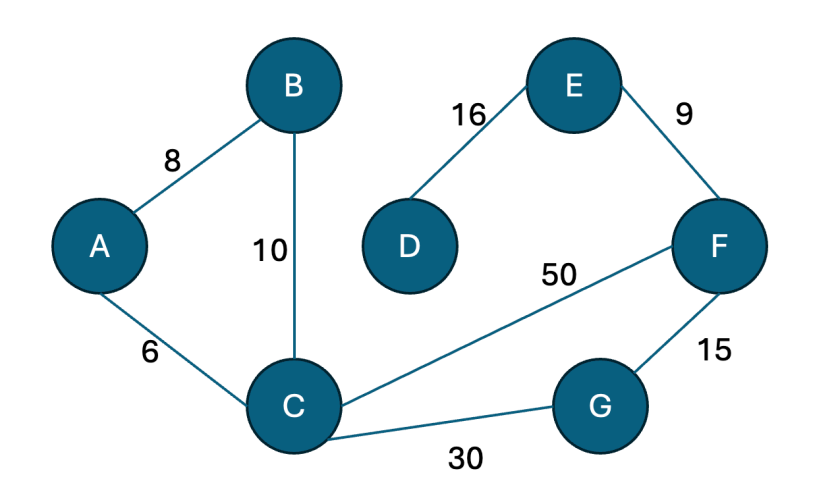
\includegraphics[width=0.6\textwidth]{task1.png} % 插入图片,设置宽度为文本宽度的一半
        % \caption{示例图片} % 图片的标题
        \label{fig:example} % 图片的标签,用于引用
    \end{figure}

    \subsection*{Task 1.1}
    由BFS算法,我们可以得到,从A点到D点的路径为:\textbf{A, C, F, E, D},\[\text{cost} = 6 + 50 + 9 + 16 = 81 \]

    \subsection*{Task 1.2}
    由DFS算法可得,从A点到D点的路径为:\textbf{A, C, G, F, E, D},\[\text{cost} = 6 + 30 + 15 + 9 + 16 = 76 \]

    \subsection*{Task 1.3}
    由UCS算法可得,从A点到D点的路径为:\textbf{A, C, G, F, E, D},\[\text{cost} = 6 + 30 + 15 + 9 + 16 = 76 \]

    \newpage
    \section*{Problem 2}
    \begin{figure}[h]
        \centering
        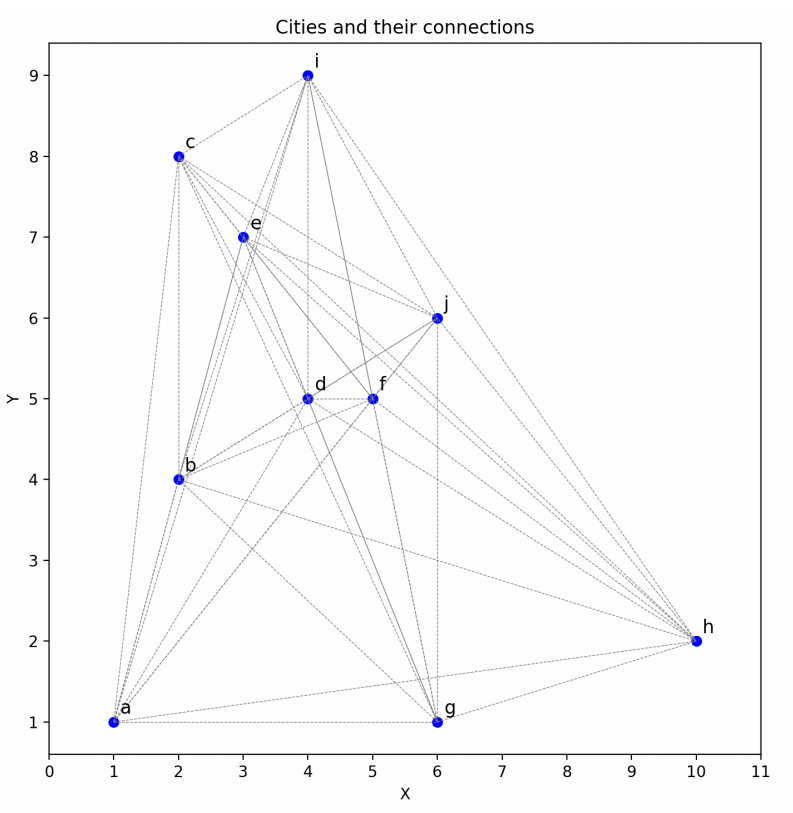
\includegraphics[width=0.6\textwidth]{task2.png} % 插入图片,设置宽度为文本宽度的一半
        % \caption{示例图片} % 图片的标题
        \label{fig:example} % 图片的标签,用于引用
    \end{figure}

    \subsection*{Task 2.1}
    由欧几里得距离公式得两个城市之间的距离为:
    \[ D_{ij} = \sqrt{(x_i - x_j)^2 + (y_i - y_j)^2} \]
    目标是找到一条经过所有城市的最短路径,且每个城市只能经过一次。
    因此,可以建立数学模型:最优路径\(R = (p_0, p_1, \cdots, p_{n-1})\): 
    \[\min f(R) = \sum_{p = 1}^{n - 1} D_{p, p+1}\]
    其中 \( n \) 表示城市的数量 \( p \)表示城市。约束条件为:
    \begin{itemize}
        \item 每个城市必须被访问一次。
        \item 必须经过所有城市。
    \end{itemize}

    \subsection*{Task 2.2}
    根据task2.1,可得\[ \text{the cost of the 'abcdefghij' path} = \sum D_{ij} = 36.904 \]
    \[ \text{the cost of the 'afhbecgijd' path} = \sum D_{ij} = 46.46 \]

    \subsection*{Task 2.3}
    在遗传算法中,适应度函数用于衡量路径的优劣。对于TSP问题,适应度函数应与路径的总长度成反比,路径越短,适应度越高。

    适应度函数可表示为:
    \[
    F(x) = \frac{1}{\text{总路径长度}}
    \]
    其中 \( F(x) \) 是路径 \( x \) 的适应度,总路径长度是通过计算所有城市之间的距离和得出的。

\end{document}